\documentclass[10pt,a4paper]{article}
\usepackage[utf8]{inputenc}
%\usepackage[T1]{fontenc}
\usepackage[french]{babel}
\usepackage{enumitem}
%\frenchbsetup{StandardLists=true}
\usepackage{caption}
\usepackage{graphicx}
\usepackage{amsmath}
\usepackage{subfigure}
\usepackage{appendix}
\usepackage{listings}
\usepackage{multicol}
\usepackage{moreverb}
\usepackage{epsfig}
\usepackage{textcomp}
\usepackage[table,xcdraw]{xcolor}
\usepackage{booktabs}

    \usepackage{xcolor}
      %%%%%%%%%%%%%%%%  inclure la source %%%%%%%%%%%%%%%%%%%%
  \newcommand*\styleC{\fontsize{9}{10pt}\usefont{T1}{cmtt}{m}{n}\selectfont }
  \newcommand*\styleD{\fontsize{9}{10pt}\usefont{T1}{cmtt}{m}{n}\selectfont }

      \makeatletter
      % on fixe le langage utilisé
      \lstset{language=matlab, breaklines=true}
      \edef\Motscle{emph={\lst@keywords}}
      \expandafter\lstset\expandafter{%
       \Motscle}
      \makeatother


      \definecolor{Vvert}{rgb}{0.133,0.545,0.133}

      \lstset{emphstyle=\color{blue}, % les mots réservés de matlab en bleu
      basicstyle=\styleC,
      keywordstyle=\cmtt,
      commentstyle=\color{Vvert}\styleD, % commentaire en gris
      numberstyle=\tiny\color{red},
      numbers=left,
      numbersep=10pt,
      lineskip=0.7pt,
      showstringspaces=false}
      %  % inclure le fichier source
      \newcommand{\FSource}[1]{%
      \lstinputlisting[texcl=true]{#1}
      }

\setlength{\textwidth}{16cm} % Largeur du texte
\setlength{\textheight}{24cm} % Hauteur du texte
\setlength{\evensidemargin}{-0.2cm} % Taille des marges pour les pages paires
\setlength{\oddsidemargin}{-0.2cm} % Taille des marges pour les pages impaires
\setlength{\topmargin}{-1.5cm} % Taille de l'ent\^ete

\title{PR307 Smart-EcoBox : \\ Planning GLRT}
\author{}

\begin{document}
\maketitle

%%%%%%%%%%%%%%%%%%%%%%%%%%%%%%%%%%%%%%%%%%%%%%%%%%%%%%%%%%%%%%%%%%%%%%%%%%%

\section{Choix des technologies}

Nos contraintes pour les données sont les suivantes :
\begin{itemize}[label=$\bullet$]
    \item La transmission des données est synchrone (les données vont être transmises successivement).
    \item Les données sont triées, opérations de jointures sur les tables $\rightarrow$ Besoin de base de données relationnelles.
    \item Les technologies doivent consommer le moins de ressources possibles pour fonctionner sur un dispositif tel qu'un Rasperry Pi.
\end{itemize}   

   \subsection*{Propositions de technologies :}
   
\begin{itemize}[label=$\bullet$]
    \setlength\itemsep{1em}
    \item \textbf{Base de données SQLite : }Cette technologie légère et relationnelle peut être contenue dans un seul fichier. 
    \item \textbf{Serveur Nginx : }Ce serveur demande peu de resources et s'adapte aux bases relationnelles.
    \item \textbf{Langages PHP : }Ce langage natif est caractéristique du domaine de développement Web et s'adapte au serveur énoncé précédemment.
    \item \textbf{JavaScript, Angular JS, JQuery : } Ces technologies vont permettre de réaliser le code client où seront affichés les différentes courbes des grandeurs physiques, les différents appareils en route et les différentes notifications par rapport aux données reçues du serveur web.
    \item \textbf{C++ :} Comme l'équipe ISNC l'utilise, l'interaction entre le récepteur/interprète et la base de données se fera dans ce langage . 
\end{itemize}

%%%%%%%%%%%%%%%%%%%%%%%%%%%%%%%%%%%%%%%%%%%%%%%%%%%%%%%%%%%%%%%%%%%%%%%%%%%

\section{Description Planning GLRT}

\begin{itemize}[label=$\bullet$]
    \setlength\itemsep{1em}
    
    \item \textbf{ Lien entre le récepteur/interprète et la base de données : Karim Toufique
    \\ $\rightarrow$ Délai: 14 novembre}\\
    Insertion des données de l'interprète/récepteur dans la base de données. 
    
    \item \textbf{Lien entre la base de données et le client web via le serveur : Karim Toufique 
    \\$\rightarrow$ Délai: 21 novembre}\\
    Organisation des réponses pouvant être effectuées par le serveur pour le client. Cela a pour but de transmettre les données fournies par la base de données au client. De même, le serveur doit répondre aux requêtes de modifications du client.
    
    \item \textbf{Client Web : Vues, Ergonomie et Calculs : Benjamin Rambaud et Marc Prats 
    \\$\rightarrow$ Délai: 28 novembre}\\
    Cette partie permet d'afficher toutes les informations dont l'utilisateur a besoin. Les courbes des grandeurs physiques, les notifications, les appareils présents ainsi que leur état sont présentés. L'ergonomie de l'interface est également un enjeu de cette partie.  
\end{itemize}

\vspace{1em}
\textbf{Remarques :} Il faut fournir une version 0 fonctionnelle et minimaliste le plus tôt possible.

%%%%%%%%%%%%%%%%%%%%%%%%%%%%%%%%%%%%%%%%%%%%%%%%%%%%%%%%%%%%%%%%%%%%%%%%%%%

\section{Backlog Produit}

US: User Stories

\begin{enumerate}[label=\bfseries US\arabic* :]
    \item L'utilisateur doit pouvoir se connecter pour accéder aux services.
    \item L'utilisateur doit pouvoir accéder aux différentes courbes des différentes grandeurs physiques( température, débit d'eau, consommation électrique).
    \item L'utilisateur doit pouvoir accéder aux différentes notifications.
    \item L'utilisateur doit pouvoir accéder à la visualisations des appareils et leur état.
    \item L'utilisateur doit pouvoir corriger l'identification du capteur ou son état.
\end{enumerate}

\section{Tâches}

 \begin{figure}[h]
     \centering % centrer l'image
     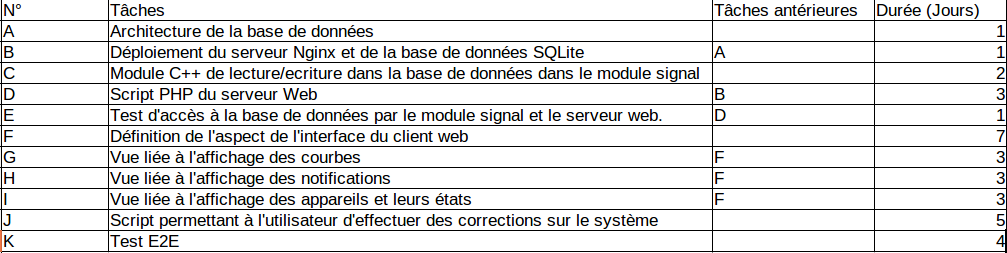
\includegraphics[scale=0.5]{matrice.png}
     \caption{Matrice des dépendances}  % Titre
 \end{figure}

%%%%%%%%%%%%%%%%%%%%%%%%%%%%%%%%%%%%%%%%%%%%%%%%%%%%%%%%%%%%%%%%%%%%%%%%%%%

\begin{thebibliography}{10}
    \bibitem{sqlite}
    Site officiel de sqlite : \emph{http://www.sqlite.org/}
    \bibitem{nginx}
    Site officiel de nginx : \emph{http://www.nginx.org/}
    \bibitem{wiki}
    Comparaison lighttpd VS nginx :  \emph{http://www.wikivs.com/wiki/lighttpd\_vs\_nginx}
\end{thebibliography}

\end{document}